% Data flow diagram
% Author: David Fokkema
\documentclass{article}
\usepackage[margin=0.5in]{geometry}
\usepackage{mathtools}
\usepackage{tikz}
\usetikzlibrary{arrows}

% Modified from http://www.texample.net/tikz/examples/data-flow-diagram/

% Defines a `datastore' shape for use in DFDs.  This inherits from a
% rectangle and only draws two horizontal lines.
\makeatletter
\pgfdeclareshape{algoprocess}{
  \inheritsavedanchors[from=rectangle]
  \inheritanchorborder[from=rectangle]
  \inheritanchor[from=rectangle]{center}
  \inheritanchor[from=rectangle]{base}
  \inheritanchor[from=rectangle]{north}
  \inheritanchor[from=rectangle]{north east}
  \inheritanchor[from=rectangle]{east}
  \inheritanchor[from=rectangle]{south east}
  \inheritanchor[from=rectangle]{south}
  \inheritanchor[from=rectangle]{south west}
  \inheritanchor[from=rectangle]{west}
  \inheritanchor[from=rectangle]{north west}
  \backgroundpath{
    %  store lower right in xa/ya and upper right in xb/yb
    \southwest \pgf@xa=\pgf@x \pgf@ya=\pgf@y
    \northeast \pgf@xb=\pgf@x \pgf@yb=\pgf@y
    \pgfpathmoveto{\pgfpoint{\pgf@xa}{\pgf@ya}}
    \pgfpathlineto{\pgfpoint{\pgf@xb}{\pgf@ya}}
    \pgfpathmoveto{\pgfpoint{\pgf@xa}{\pgf@yb}}
    \pgfpathlineto{\pgfpoint{\pgf@xb}{\pgf@yb}}
 }
}
\makeatother

\begin{document}
\begin{center}
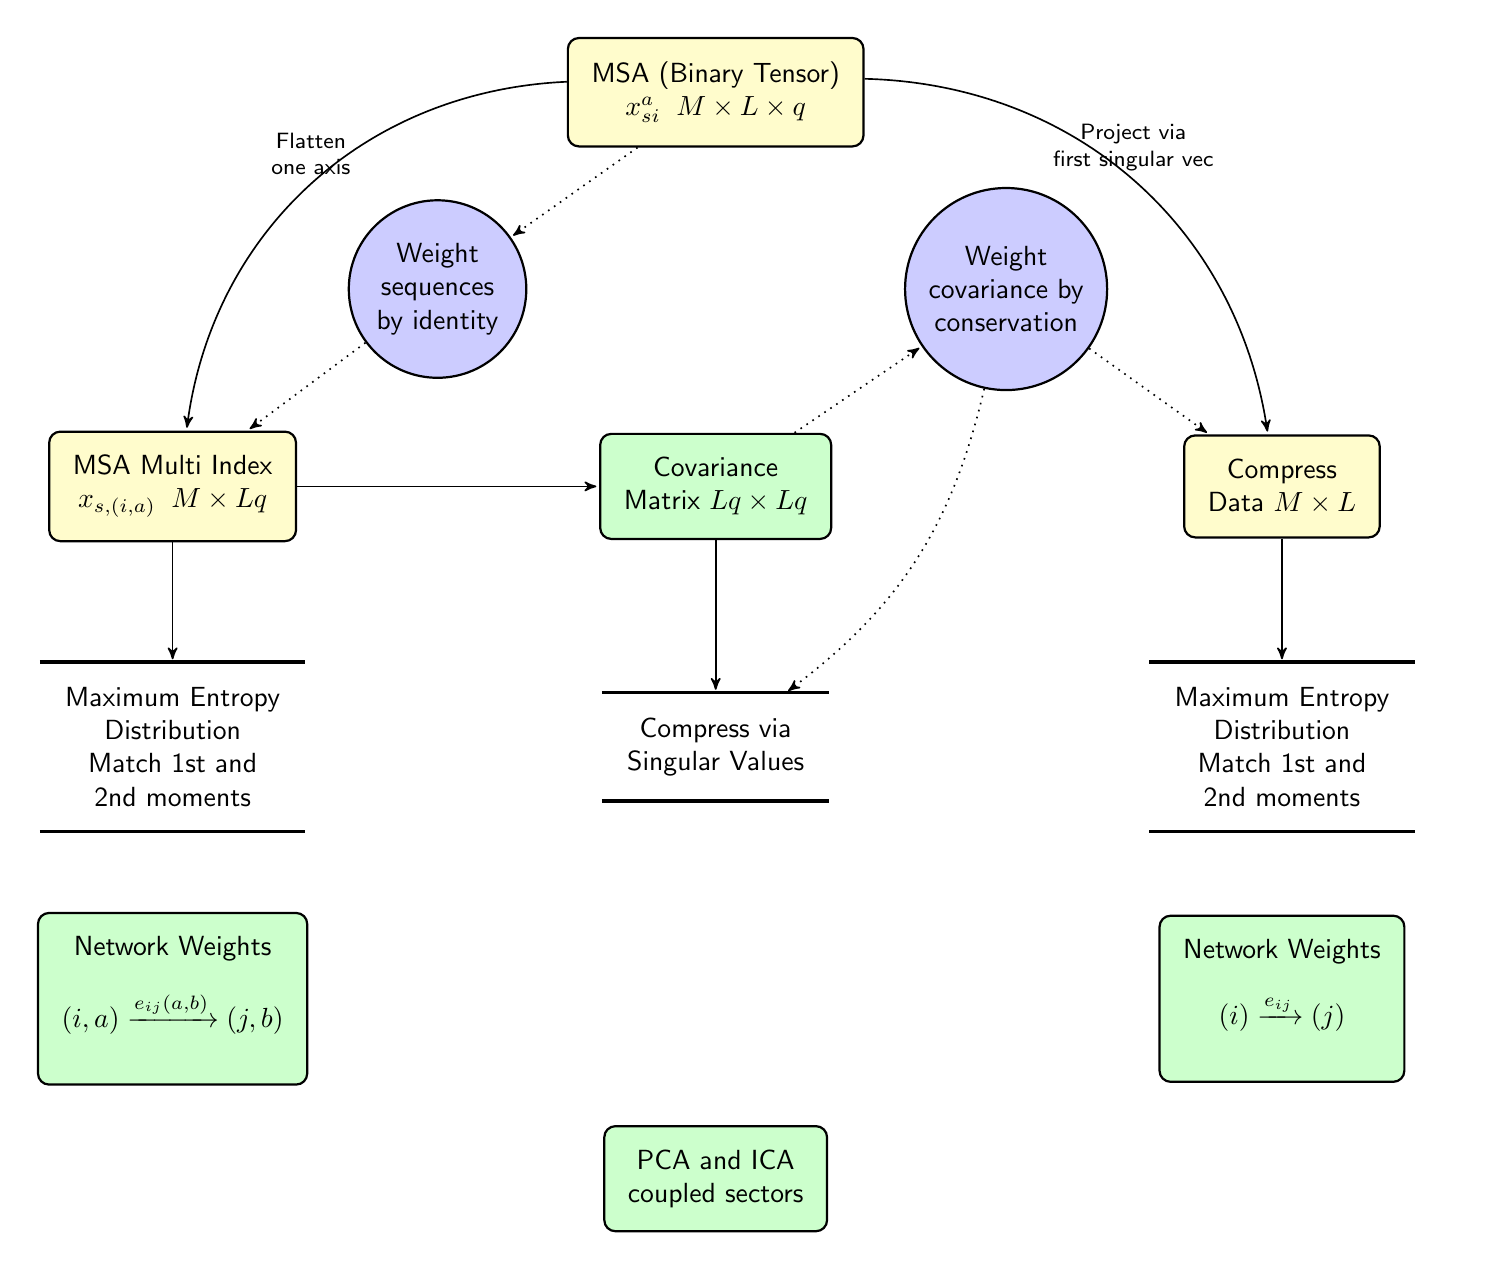
\begin{tikzpicture}[
  font=\sffamily,
  every matrix/.style={ampersand replacement=\&,column sep=.5cm,row sep=.5cm},
  datamat/.style={draw,thick,rounded corners,fill=yellow!20,inner sep=.3cm},
  process/.style={draw,thick,circle,fill=blue!20},
  calcmat/.style={datamat,fill=green!20},
  algoprocess/.style={draw,very thick,shape=algoprocess,inner sep=.3cm},
  to/.style={->,>=stealth',shorten >=1pt,semithick,font=\sffamily\footnotesize},
  todots/.style={->,dotted,>=stealth',shorten >=1pt,semithick,font=\sffamily\footnotesize},
  every node/.style={align=center}]
% Position the nodes using a matrix layout
  \matrix{

    \&
    \&  \node[datamat] (MSA) {
            MSA (Binary Tensor) \\ $x_{si}^a \; \; M\times L \times q$
        }; 
    \&
    \& \\

    \& \node[process] (weightseqid) {
                Weight \\ sequences \\ by identity
        }; 
    \& 
    \& \node[process] (weightcons) {
                Weight \\ covariance by \\ conservation
        }; 
    \& \\

    \node[datamat] (FlattenMSA) {
            MSA Multi Index \\ $x_{s, (i,a)}\;\; M\times Lq$
        };  
    \& 
    \& \node[calcmat] (CovMat) {
            Covariance\\Matrix $Lq\times Lq$
        };
    \&
    \& \node[datamat] (DataProj) {
            Compress\\Data $M\times L$
        }; \\

    % new line in matrix
    \\
    \\

    \node[algoprocess] (MaxEntBig) {
            Maximum Entropy \\Distribution\\ Match 1st and \\ 2nd moments
        };  
    \& 
    \& \node[algoprocess] (CompressCov) {
            Compress via\\Singular Values
        };
    \&
    \& \node[algoprocess] (MaxEntSmall) {
            Maximum Entropy \\Distribution\\ Match 1st and \\ 2nd moments
        };  
    \& \\

    \\

    \node[calcmat] (NetworkBig) {
            Network Weights \\ \\ $(i,a) \xrightarrow{e_{ij}(a,b)} (j,b)$ \\ 
        };  
    \& 
    \&
    \&
    \& \node[calcmat] (NetworkSmall) {
            Network Weights \\ \\ $(i) \xrightarrow{e_{ij}} (j)$ \\ 
        };  
    \\

    \& 
    \& \node[calcmat] (Sectors) {
            PCA and ICA \\ coupled sectors
        };
    \& \\
  };

  % Draw the arrows between the nodes and label them.
  \draw[to]     (MSA) to[bend right=40] 
                    node[midway,above] {Flatten \\ one axis} 
                (FlattenMSA);
  \draw[todots] (MSA)           --  (weightseqid);
  \draw[todots] (weightseqid)   --  (FlattenMSA);
  \draw[to]     (FlattenMSA)    --  (CovMat);
  \draw[todots] (CovMat)        --  (weightcons);
  \draw[to]     (MSA) to[bend left=40] 
                    node[midway,above] {Project via \\ first singular vec} 
                (DataProj);
  \draw[todots] (weightcons)    --  (DataProj);
  \draw[to]     (FlattenMSA)    --  (MaxEntBig);
  \draw[to]     (CovMat)        --  (CompressCov);
  \draw[todots] (weightcons)    to[bend left=20]  (CompressCov);
  \draw[to]     (DataProj)      --  (MaxEntSmall);
\end{tikzpicture}
\end{center}
\end{document}
